%; whizzy paragraph -pdf xpdf -latex ./whizzypdfptex.sh
%; whizzy-paragraph "^\\\\begin{frame}"
% latex beamer presentation.
% platex, latex-beamer でコンパイルすることを想定。 

%     Tokyo Debian Meeting resources
%     Copyright (C) 2009 Junichi Uekawa
%     Copyright (C) 2010 Nobuhiro Iwamatsu

%     This program is free software; you can redistribute it and/or modify
%     it under the terms of the GNU General Public License as published by
%     the Free Software Foundation; either version 2 of the License, or
%     (at your option) any later version.

%     This program is distributed in the hope that it will be useful,
%     but WITHOUT ANY WARRANTY; without even the implied warranty of
%     MERCHANTABILITY or FITNESS FOR A PARTICULAR PURPOSE.  See the
%     GNU General Public License for more details.

%     You should have received a copy of the GNU General Public License
%     along with this program; if not, write to the Free Software
%     Foundation, Inc., 51 Franklin St, Fifth Floor, Boston, MA  02110-1301 USA

\documentclass[cjk,dvipdfmx,12pt]{beamer}
\usetheme{Tokyo}
\usepackage{monthlypresentation}
%  preview (shell-command (concat "evince " (replace-regexp-in-string "tex$" "pdf"(buffer-file-name)) "&"))
%  presentation (shell-command (concat "xpdf -fullscreen " (replace-regexp-in-string "tex$" "pdf"(buffer-file-name)) "&"))
%  presentation (shell-command (concat "evince " (replace-regexp-in-string "tex$" "pdf"(buffer-file-name)) "&"))

%http://www.naney.org/diki/dk/hyperref.html
%日本語EUC系環境の時
\AtBeginDvi{\special{pdf:tounicode EUC-UCS2}}
%シフトJIS系環境の時
%\AtBeginDvi{\special{pdf:tounicode 90ms-RKSJ-UCS2}}

\title{東京エリア Debian 勉強会}
\subtitle{資料}
\author{上川純一 dancer@debian.org\\IRC nick: dancerj}
\date{2010年03月20日}
\logo{
\includegraphics[width=8cm]{image200607/openlogo-light.eps}}

\begin{document}

\frame{\titlepage{}}

\emtext{設営準備にご協力ください}

\begin{frame}
 \frametitle{勉強会の連絡事項}
\begin{minipage}[t]{0.45\hsize}
  \begin{itemize}
   \item 注意事項
	 \begin{itemize}
	  \item 飲食?
	 \end{itemize}
  \end{itemize}
\end{minipage} 
\begin{minipage}[t]{0.45\hsize}
 \begin{itemize}
  \item ニューラルネットワークで画像を分類してみた
  \item weka
  \item libfftw
  \item man-db 深追い
  \item dpkg v3 quilt
 \end{itemize}
\end{minipage}
\end{frame}

\begin{frame}{Hack Cafe}
 最近ハックカフェしてますか?
 \url{http://twitter.com/debian_hackcafe}\\
\end{frame}

\emtext{事前課題}

\begin{frame}{事前課題}
\begin{enumerate}
 \item 好きな日本語Manページ
 \item ニューラルネットワークで解決できる問題
\end{enumerate}
\end{frame}

{\footnotesize

% this is a prework file.

}

% ------------------------------------------------------------------------------
\emtext{ニューラルネットワークで画像を分類してみた}
% ------------------------------------------------------------------------------

% ------------------------------------------------------------------------------
\emtext{Debianでwekaを使ってみる}
% ------------------------------------------------------------------------------

% ------------------------------------------------------------------------------
\emtext{Debianでlibfftwを使ってみる}
% ------------------------------------------------------------------------------

\begin{frame}{はじめに}
音声データの解析、とりあえずまず FFT をかける。

DebianでFFT処理をするためのステップとして、音声データのロードとFFT処理が
ある。
コードを書いてみるのに、Debianパッケージを活用する

\begin{itemize}
 \item 音声データの作成: 適当なツールを使う
 \item 音声データのロード: sndfile 
 \item FFT処理: libfftw
 \item 結果の処理: R
\end{itemize}
\end{frame}

\begin{frame}[containsverbatim]{材料となる音声データを準備}

aeolus を vkeybd で midi 制御しつつ、ecasound で jack 経由で音声を録音。
sweep で後で適切なサイズに切り出す。

\begin{commandline}
$ qjackctl &
$ aeolus &
$ vkeybd &
$ ecasound -i jack -o test.wav
ctrl-C で中断
$ sweep test.wav # 適当に編集
$ file ra-mono.wav  # 切り出した結果を確認
ra-mono.wav: RIFF (little-endian) data, WAVE audio, 
Microsoft PCM, 16 bit, mono 44100 Hz
\end{commandline}
 
\end{frame}

\begin{frame}[containsverbatim]{必要なパッケージをインストール}
 
\begin{commandline}
$ apt-get install libfftw3-dev libsndfile1-dev
\end{commandline}

\end{frame}

\begin{frame}[containsverbatim]{コードを書いてみた1: sndfile}

sndfile の提供するAPIを使い、 double の配列に音声データ(wav ファイル)を
読み込む。

\begin{commandline}
  SF_INFO sfinfo = {0, 0, 0, 0, 0, 0};
  SNDFILE* s = sf_open(filename, SFM_READ, &sfinfo);
  double* data = malloc(sizeof(double) * size);
  sf_readf_double(s, data, size / sfinfo.channels);
  study_sound(data, size / sfinfo.channels);
  sf_close(s);
\end{commandline} 
\end{frame}

\begin{frame}[containsverbatim]{コードを書いてみた2: FFT}

FFTW の提供するAPIを使い、double の配列をFFT処理、結果を複素数の配列にい
れる。

\begin{commandline}
  fftw_complex* spectrum;
  fftw_plan p;
  spectrum = (fftw_complex*) fftw_malloc(
    sizeof(fftw_complex) * (size / 2 + 1));
  p = fftw_plan_dft_r2c_1d(size, data, spectrum, FFTW_ESTIMATE);
  fftw_execute(p);
\end{commandline} 
\end{frame}

\begin{frame}[containsverbatim]{Rでグラフにしてみた}

結果を適当にcsvで出力して、グラフにして分析。
簡単に処理するために、Rを使う。

\begin{commandline}
$ R
> sine <- read.csv("sine.csv")
> ra <- read.csv("ra.csv")
> postscript("sine.eps", horizontal=FALSE, height=3, width=3)
> plot(sine$i, sine$abs, xlim=c(400,500), ylim=c(0,22000), 
    type="l")
> dev.off()
> postscript("ra.eps", horizontal=FALSE, height=3, width=3)
> plot(ra$i, ra$abs, xlim=c(0,2000), ylim=c(0,100), type="l")
> dev.off()

\end{commandline} 

\end{frame}

\begin{frame}{実行結果}

 \includegraphics[width=0.5\hsize]{image201003/sine.eps}
 \includegraphics[width=0.5\hsize]{image201003/ra.eps}
 
\end{frame}

% ------------------------------------------------------------------------------
\emtext{man-db}
% ------------------------------------------------------------------------------

% ------------------------------------------------------------------------------
\emtext{dpkg v3 quilt}
% ------------------------------------------------------------------------------

\begin{frame}{次回の勉強会}

\begin{itemize}
 \item 2010年4月?日: どこ?
\end{itemize}
 
\end{frame}

\end{document}

;;; Local Variables: ***
;;; outline-regexp: "\\([ 	]*\\\\\\(documentstyle\\|documentclass\\|emtext\\|section\\|begin{frame}\\)\\*?[ 	]*[[{]\\|[]+\\)" ***
;;; End: ***
